\documentclass[11pt, letterpaper]{article}
\usepackage[utf8]{inputenc}
\usepackage{graphicx}
\usepackage[spanish]{babel}
\graphicspath{{imageneslatex/}}
\usepackage{parskip}

\title{Estacion de Carga }
\author{Ray Marcelo Ibarra }
\date{\today}



\begin{document}
\maketitle

\begin{center}  
    \textbf{introduccion}
\end{center}
La idea principal nace por el uso y la gran importancia que le damos a los celulares esta herramienta fundamental 
, es por ello que ideamos la forma de poder cargar esta herramienta y dar a entender a las personas que pueden salir 
de sus casas sin preocupacion de que se queden sin bateria 
una vez aclarado este punto tengamos en cuenta el beneficio que trae este proyecto 
tratando de cambiar y mejorar lo que antes se nos hacia muy tedioso que era llevar 
cargador y buscar algun puerto de carga y tambien la necesidad de buscar un lugar que 
tenga estos puertos este problema se vio por mucho tiempo
\\ \\
\\ \\
\\ \\
\\ \\
\\ \\
\\ \\
\\ \\
\\ \\
\\ \\
\tableofcontents

\section{componentes del proyecto}
\begin{center}
    \textbf{1.1.-arduino uno}
\end{center}
Arduino Uno es una placa de desarrollo de hardware libre diseñada para facilitar la creación de 
proyectos electrónicos interactivos.
Fue lanzada en 2010 y es una de las placas más populares de la familia Arduino.\\
La placa Arduino Uno utiliza un microcontrolador ATmega328P de Atmel y tiene una serie de pines que se pueden 
programar para leer sensores, controlar 
actuadores y comunicarse con otros dispositivos. 
La placa también tiene un puerto USB que se utiliza para 
cargar programas en el microcontrolador
 y para comunicarse con el ordenador.\\



\begin{figure}[h!]
    \centering
    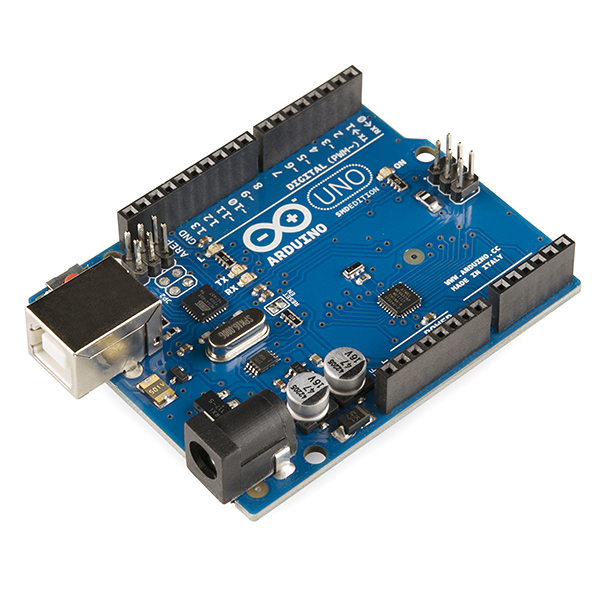
\includegraphics[height=4cm]{Arduino_Uno_-_R3.jpg}
    \caption{arduino uno }
    \label{fig:arduino uno }
\end{figure} 
arduino 
\\ \\
\\ \\
\\ \\
\\ \\
\\ \\
\begin{center}

    \textbf{1.2.- microcontrolador ATmega328P}
\end{center}
El microcontrolador ATmega328P es un chip de 8 bits fabricado por la empresa de semiconductores Atmel, ahora propiedad de Microchip Technology. 
Es uno de los microcontroladores más populares y ampliamente utilizados en el mundo de la electrónica y la programación debido a su facilidad de uso, 
bajo costo y gran cantidad de características y funcionalidades.
El ATmega328P cuenta con una CPU de 8 bits con una velocidad de reloj máxima de 20 MHz, memoria flash de 32 KB para almacenar programas y datos,
2 KB de memoria SRAM, y 1 KB de EEPROM. También incluye una amplia variedad de periféricos, como puertos de entrada y salida digitales, 
puertos analógicos, temporizadores, contadores, PWM, UART, SPI e interfaz I2C, entre otros.
Este microcontrolador es ampliamente utilizado en proyectos de electrónica, desde aplicaciones simples hasta proyectos más complejos. 
Es comúnmente utilizado en la creación de proyectos de robótica, controladores de motores, sistemas de sensores y dispositivos de automatización 
del hogar, entre otros.
El ATmega328P es compatible con varios entornos de desarrollo, como el popular Arduino IDE, lo que lo hace fácil de programar y utilizar 
para los aficionados a la electrónica y los desarrolladores. Además, el chip es compatible con diferentes tipos de hardware y módulos adicionales, 
lo que lo convierte en una opción flexible para proyectos personalizados.
En resumen, el microcontrolador ATmega328P es una excelente opción para una amplia variedad de aplicaciones electrónicas 
debido a su facilidad de uso, características y funcionalidades, y compatibilidad con diferentes entornos de desarrollo y hardware adicional.
\begin{figure}[h!]
    \centering
    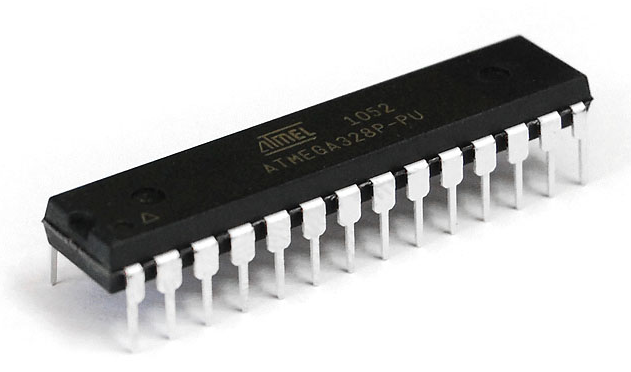
\includegraphics[height=4cm]{atmega328p-pu.png}
    \caption{ATmega328P }
    \label{fig:ATmega328P }
\end{figure} 
ATmega328P\\
estos son los componentes principales y requeridos obligatoriamente 
para poder realizar este proyecto
\\ \\
\\ \\
\begin{center}

    \textbf{1.3.-cables de conexion para Arduino}
\end{center}
Los cables puente son cables con dos extremos de conexión que se utilizan para conectar 
iferentes pines de la placa de Arduino a otros componentes electrónicos. Son muy útiles en proyectos de prototipado y en la creación 
de circuitos electrónicos.
Los cables puente vienen en diferentes
tamaños y longitudes, y generalmente están hechos de alambre de cobre con una capa aislante de plástico. 
Pueden ser macho-macho, macho-hembra o hembra-hembra, según las necesidades de conexión del proyecto.
Los cables puente se utilizan para realizar conexiones temporales y prototipar circuitos electrónicos de manera rápida y sencilla. 
Por ejemplo, si deseas conectar un sensor a la placa de Arduino, puedes utilizar un cable puente para conectar el pin de salida del sensor 
al pin de entrada de la placa de Arduino. De esta manera, el sensor puede enviar datos a la placa de Arduino y el programa que se ejecuta
en ella puede procesarlos.
\begin{figure}[h!]
    \centering
    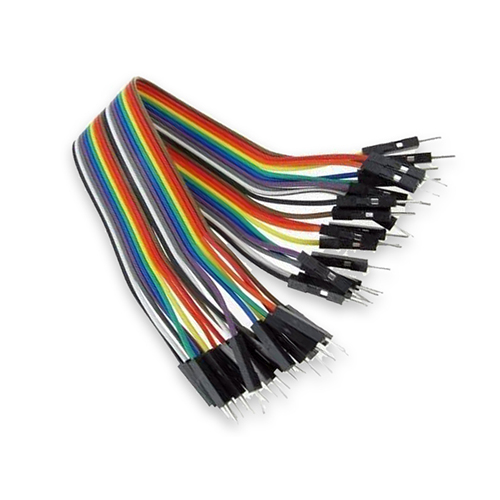
\includegraphics[height=4cm]{cables-arduino.jpg}
    \caption{cables de conexion}
    \label{fig:cables de conexion }
\end{figure}
cables de conexion
\\ \\ 
\\ \\ 
\\ \\ 
\begin{center}
    \textbf{1.4.-dasdasfdadadasfa}
\end{center}






\section{armado del proyecto }
Este proyecto consto de meses de trabajo para poder realizarlo
estuvimos pensando en el mecanismo de este asi como falta 
mejorar en algunos aspectos tambien implementar mas cosas 
se realizara todo esto con el pasar del tiempo para poder comenzar 
con este proyecto debemos conseguir las piezas necesarias para el armado 
el codigo aun no puedo hacerlo publico necesita algunas mejoras conectamos el arduino
de la siguiente forma con las piezas que tenemos 
\section{fallas y mejoras para poder realizarse}
\section{gasto y costo del proyecto}
\section{conclusion}
\end{document}